\documentclass[journal]{IEEEtran}
\usepackage[usenames]{color}
\usepackage{epsfig}
\usepackage{graphics}
\usepackage{caption}
\usepackage{amsmath}
\usepackage{amssymb}
\usepackage{multirow}
\usepackage{cite}
\usepackage{array}
\usepackage{url}
\usepackage{lineno}
\usepackage{graphicx}
\usepackage{setspace}
\usepackage{tikz}
\usepackage{hhline}
\usepackage{mathtools}
\usepackage{caption}
\usepackage{xcolor}
\usepackage[letterpaper]{geometry}
\geometry{verbose,tmargin=0.55in,bmargin=1.0in,lmargin=0.65in,rmargin=0.65in}
\setlength{\headheight}{48pt}
\setlength{\headsep}{14pt}

% 中文支持（需使用XeLaTeX编译）
\usepackage{xeCJK}
\setCJKmainfont{Noto Serif CJK SC}         % 正文：思源宋体
\setCJKsansfont{Noto Sans CJK SC}          % 无衬线：思源黑体
\setCJKmonofont{Noto Sans Mono CJK SC}     % 等宽字体

\renewcommand{\abstractname}{\textcolor{violet}{\textbf{ABSTRACT / 摘要}} }
 \newcommand{\flogo}{
\includegraphics[height=40pt]{LOGO1.png}
 }

\pagenumbering{gobble}

\usepackage{fancyhdr}
\pagestyle{fancy}
\fancyhf{}
\lhead{\flogo}
\rhead{
\includegraphics[height=40pt]{LOGO2.png} \thepage}
\pagestyle{fancyplain}

	\makeatletter
\ifCLASSOPTIONjournal
\def\abstract{\@IEEEtweakunitybaselinestretch{1.15}
	\@IEEEabskeysecsize\noindent\abstractname---\relax
	\fi\@IEEEgobbleleadPARNLSP}
\makeatother


\begin{document}

	\title{\vspace*{0.5cm}\textcolor{violet}{这里是论文的中文标题，请替换为您的研究题目}
	\vspace*{0.5cm}
	}


	\author{\textbf{第一作者$^{1}$，第二作者$^{2}$，第三作者$^{1,*}$}\\
		\vspace*{0.1cm}

		在此填写作者的单位信息和资助信息 \\
		\vspace*{0.2cm}
		\small
		$^{1}$ 第一单位，城市，国家 \\
		$^{2}$ 第二单位，城市，国家 \\
		\vspace*{0.1cm}
		通讯作者：第三作者（e-mail: author@example.com）\\
		\vspace*{0.1cm}
		本研究由某某基金资助（项目编号：XXXXXXX）\\
		本文包含补充材料
		\normalsize
	}


	\twocolumn[
	\begin{@twocolumnfalse}
	\let\newpage\relax\maketitle\thispagestyle{fancy}
		\begin{abstract}
		摘要应简要概括论文的内容，并涵盖以下要点。目的：用通俗易懂的语言简要陈述所研究的问题或议题。结果：简要总结研究的结果和发现。结论：对研究结果给出简短的总结性评述。摘要摘要摘要摘要摘要摘要摘要摘要摘要摘要摘要摘要摘要摘要摘要摘要摘要摘要摘要摘要摘要摘要摘要摘要摘要摘要摘要摘要摘要摘要摘要摘要摘要摘要摘要摘要摘要摘要摘要摘要。\\
		\\
\noindent
\textcolor{violet}{\textbf{INDEX TERMS / 关键词}}  关键词一，关键词二，关键词三，关键词四，关键词五。\\
\\
\textcolor{violet}{\textbf{IMPACT STATEMENT / 影响声明}} 概括本文报告的研究工作的主要发现。
\vspace{0.5cm}

	\end{abstract}
\end{@twocolumnfalse}
]


\IEEEpeerreviewmaketitle

\section{INTRODUCTION / 引言}

本文研究了某某问题。近年来，随着某某技术的快速发展，该领域受到了广泛关注。然而，目前仍存在诸多挑战，例如某某问题尚未得到有效解决。本文提出了一种新的方法来解决上述问题。

引言部分应包含以下内容：研究背景与动机、相关工作综述、本文的主要贡献以及论文的组织结构。引言引言引言引言引言引言引言引言引言引言引言引言引言引言引言引言引言引言引言引言引言引言引言引言引言引言引言引言。

\section{RESULTS / 结果}

本节展示实验结果。表~\ref{Exp}和图~\ref{fig:examplesinglefig}分别展示了定量和定性结果。

实验结果表明，所提出的方法在多个评价指标上均优于现有的基线方法。具体而言，在指标一上提升了X\%，在指标二上提升了Y\%。结果结果结果结果结果结果结果结果结果结果结果结果结果结果结果结果结果结果结果结果结果结果结果结果结果结果。

\section{DISCUSSION / 讨论}

本节对实验结果进行讨论与分析。讨论讨论讨论讨论讨论讨论讨论讨论讨论讨论讨论讨论讨论讨论讨论讨论讨论讨论讨论讨论讨论讨论讨论讨论讨论讨论讨论讨论讨论讨论讨论讨论讨论。

\subsection{Equations / 公式}
公式应连续编号，编号用括号括起来并靠右对齐，如公式(\ref{Eq:Example})所示。

\begin{equation}
\begin{multlined}
\int_{0}^{r_{2}} F(r,\varphi)dr d\varphi=[\sigma r_{2}/(2\mu_{0})]\\
\int_{0}^{+\infty}exp(-\lambda |z_{j}-z_{i} |)\lambda^{-1} J_{1}(\lambda r_{2}) J_{0}(\lambda r_{1})d\lambda
\label{Eq:Example}
\end{multlined}
\end{equation}

请确保公式中的符号在公式出现之前或紧随其后进行定义。讨论讨论讨论讨论讨论讨论讨论讨论讨论讨论讨论讨论讨论讨论讨论。

\section{CONCLUSION / 结论}

本文提出了一种用于解决某某问题的新方法。实验结果表明，所提方法在多个基准数据集上取得了优异的性能。主要贡献总结如下：

第一，提出了某某创新方法；第二，设计了某某实验验证方案；第三，在某某数据集上验证了方法的有效性。

未来工作将进一步探索该方法在更多场景中的应用。结论结论结论结论结论结论结论结论结论结论结论结论结论结论结论。

\begin{figure}[t]
	\centering
	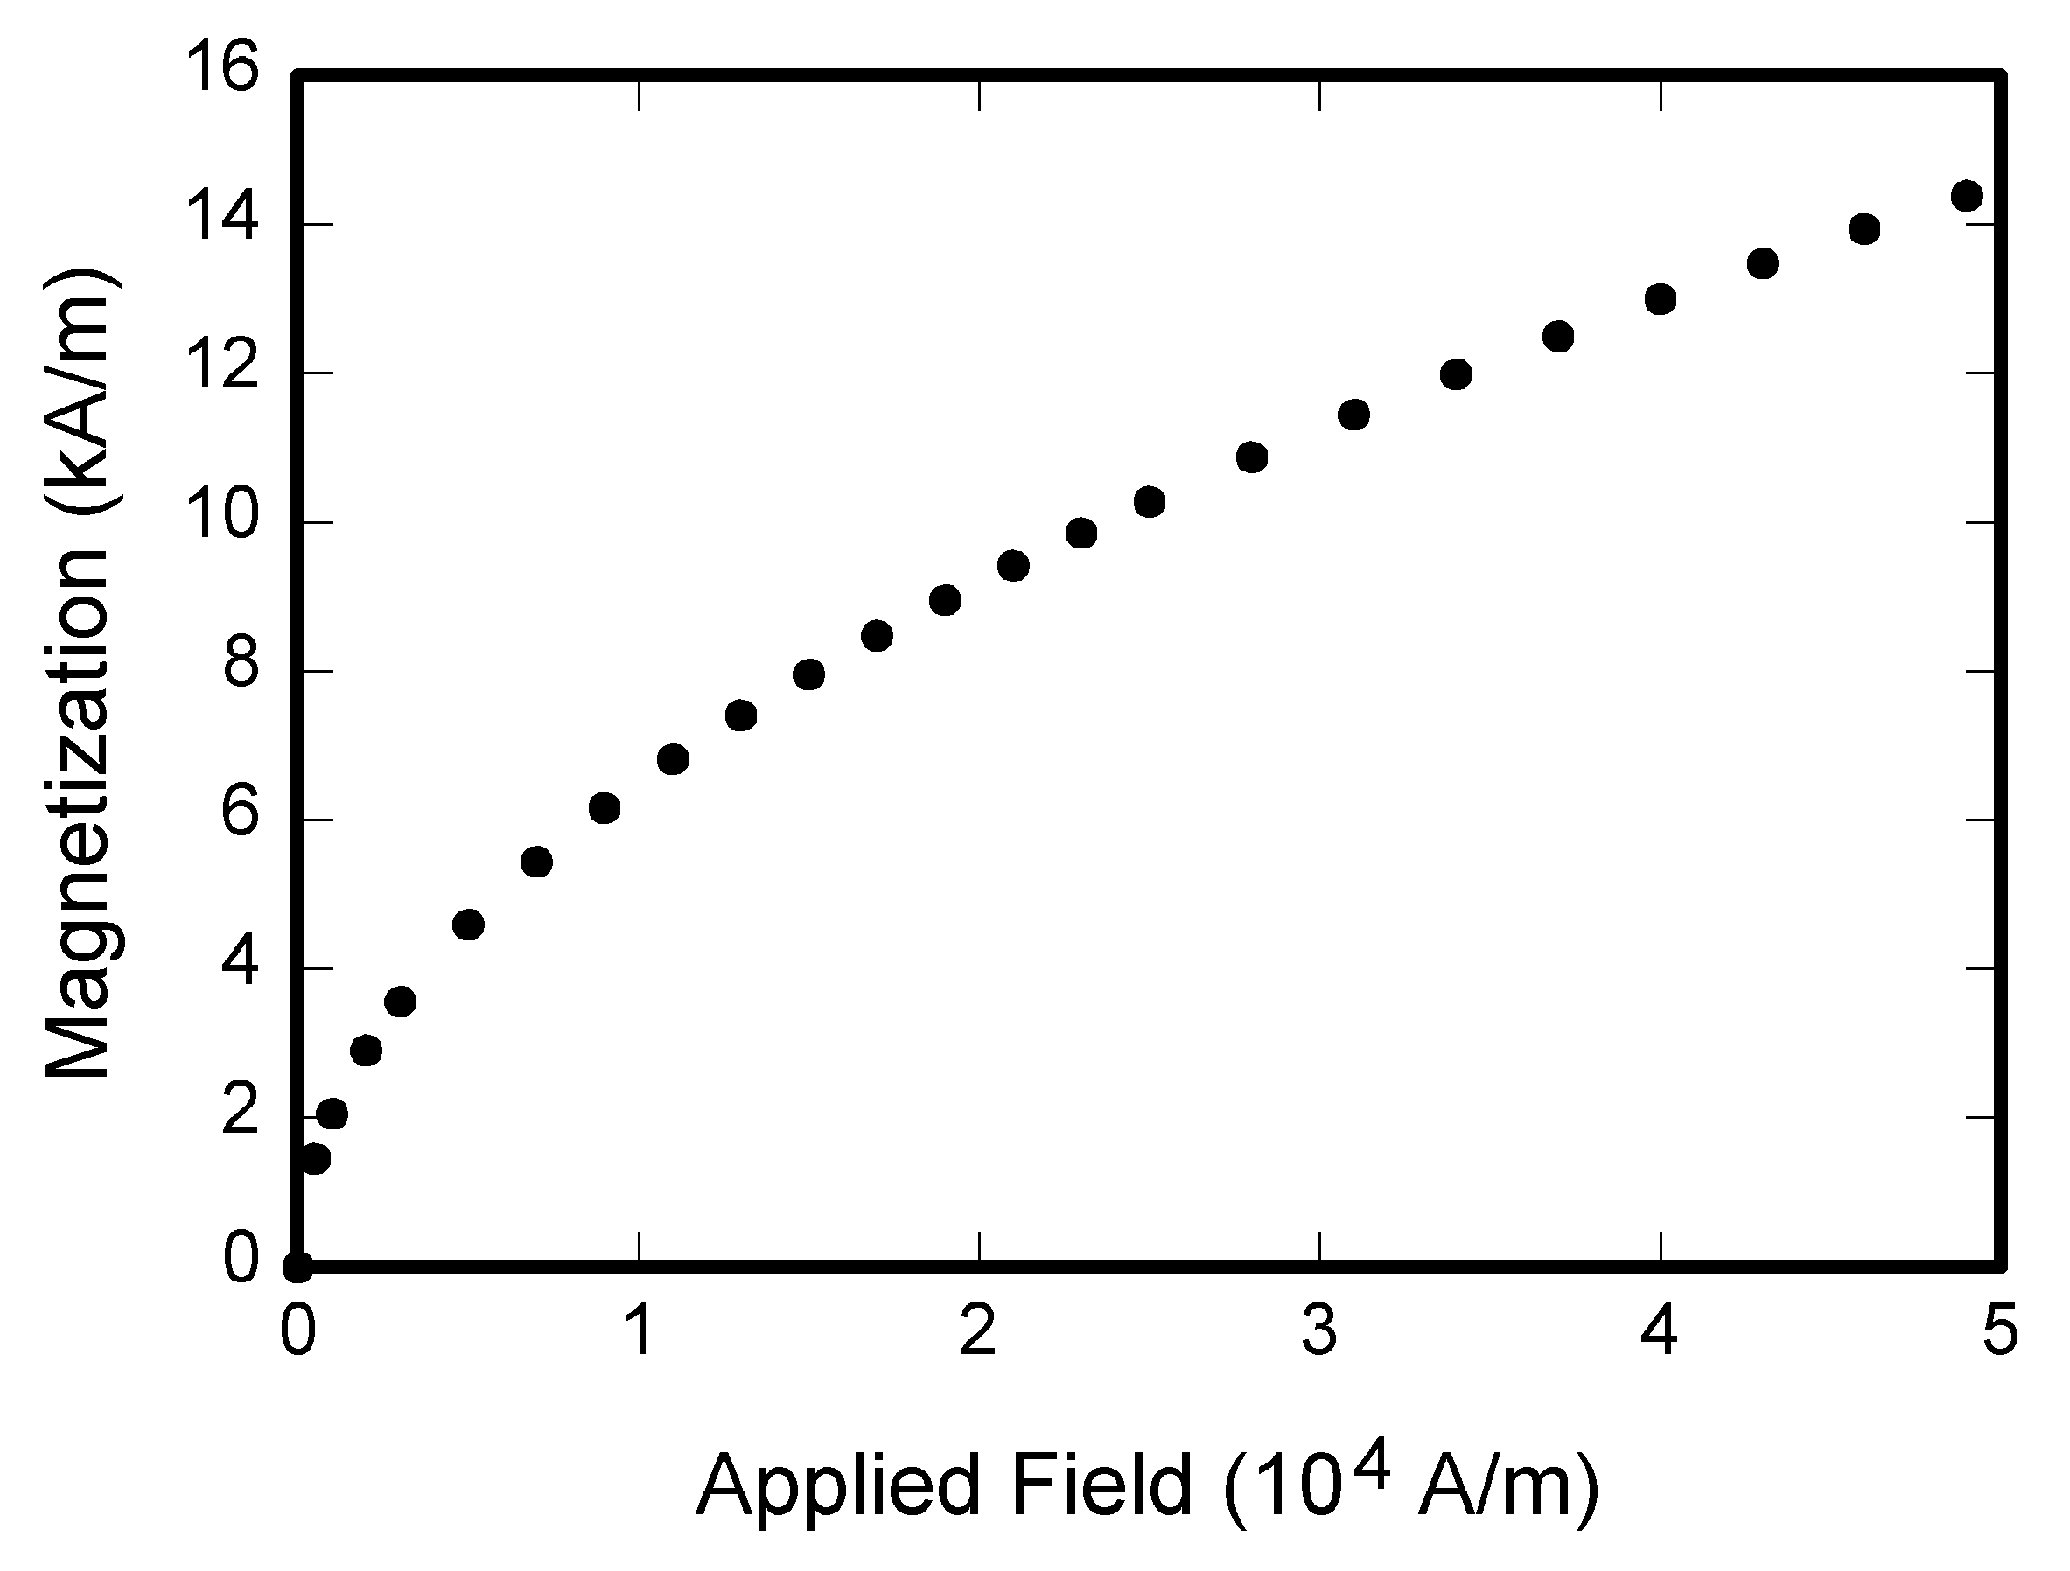
\includegraphics[width=\linewidth]{./fig1.png}
	\caption{示例图片说明。请在此处描述图片的内容和意义。}
	\label{fig:examplesinglefig}
\end{figure}


\begin{table}[ht]
	\begin{center}
		\small
		\resizebox{1\columnwidth}{!}{
			\begin{tabular}{ m{0.2\columnwidth} >{\raggedleft}m{0.3\columnwidth} m{0.5\columnwidth} }
				\multicolumn{3}{c}{\textsc{示例表格标题}} \\
				\hhline{===}
				{方法} & {指标一} & {指标二} \\
				\hline
				方法A & 85.2 & 90.1 \\
				方法B & 87.5 & 91.3 \\
				本文方法 & \textbf{92.1} & \textbf{95.6} \\
				\hhline{===}

			\end{tabular}
		}
	\end{center}
	\caption{各方法在基准数据集上的性能比较。粗体表示最优结果。}
	\label{Exp}
\end{table}
\normalsize


\section{MATERIALS AND METHODS / 材料与方法}
本节介绍实验所使用的材料与方法。材料与方法材料与方法材料与方法材料与方法材料与方法材料与方法材料与方法材料与方法材料与方法材料与方法材料与方法材料与方法材料与方法。\\

SUPPLEMENTARY MATERIAL / 补充材料\\
补充材料部分的简要说明。如有补充材料，请在此引导读者了解补充材料的内容。\\


ACKNOWLEDGEMENT / 致谢\\
致谢内容。感谢某某机构和个人对本研究的支持与帮助。


\begin{thebibliography}{1}

	\bibitem{ref1} 作者A，作者B，``论文标题一，'' \textit{期刊名称}，vol.~1，no.~1，pp.~1--10，2024。

	\bibitem{ref2} 作者C，作者D，``论文标题二，'' \textit{期刊名称}，vol.~2，no.~3，pp.~100--120，2023。

	\bibitem{ref3} 作者E，\textit{书名}。出版地：出版社，2022，pp.~50--80。

\end{thebibliography}


\end{document}